\documentclass[main.tex]{subfiles}

\begin{document}

\chapter{Second-order Systems}

So far we have seen first-order differential equations and systems of first-order ODEs.  In this chapter we introduce second-order systems, which are particularly useful for modeling Newtonian motion.

\index{Newtonian motion}
\index{Newton's law of motion}

\section{Newtonian motion}

Newton's second law of motion is often written like this:

\begin{equation}
    F = m a
\end{equation}

where $F$ is the net force acting on an object, $m$ is the
mass of the object, and $a$ is the acceleration of the object.

This equation suggests
that if you know $m$ and $a$ you can compute force, which is true,
but in most physical simulations it is the other way around:  based on a
physical model, you know $F$ and $m$, and you compute $a$.

\index{second derivative}
\index{second-order differential equation}
\index{differential equation!second-order}

So if we know acceleration as a function of time, how do we
find the position of the object, $r$?  Well, we know that acceleration
is the second derivative of position, so we can write a differential
equation

\begin{equation}
    \frac{d^2r}{dt^2} = a
\end{equation}

where $\frac{d^2r}{dt^2}$ is the second time derivative of $r$.

Because this equation includes a second derivative, it is
a second-order ODE.  {\tt ode45} can't solve the equation this form, but
by introducing a new variable, {\tt v}, for velocity, we can rewrite it
as a system of first-order ODEs:

\begin{eqnarray}
    \frac{dr}{dt} &=& v   \\
    \frac{dv}{dt} &=& a   \\
\end{eqnarray}

The first equation says that the first derivative of $r$ is $v$;
the second equation says that the first derivative of $v$ is $a$.


\section{Freefall}
\label{freefall}

As an example, let's get back to the question from Exercise~\ref{penny}:

\begin{quote}
If you drop a penny from the top of the Empire State Building, how long does it take to reach the sidewalk, and how fast it is going when it gets there?
\end{quote}

We'll start with no air resistance; then we'll add air resistance to the model and see what effect it has.

\index{air resistance}
\index{gravity}

Near the surface of the earth,
acceleration due to gravity is $-9.8$ $m/s^2$, where the minus sign
indicates that gravity pulls down.

If the object falls straight down, we can describe its position with a
scalar value $y$, representing altitude.

\index{position}
\index{velocity}
\index{rate function }
Here is a rate function we can use with {\tt ode45} to solve
this problem:

\begin{code}
function res = rate_func(t, X)
    % unpack position and velocity
    y = X(1);      
    v = X(2);      
    
    % compute the derivatives
    dydt = v;
    dvdt = -9.8;

    % pack the derivatives into a column vector
    res = [dydt; dvdt];
end
\end{code}

The rate function takes {\tt t} and {\tt X} as input variables, where the elements of {\tt X} are understood to be the position and velocity of the object.
It returns a column vector that contains {\tt dydt} and {\tt dvdt}, which
are velocity and acceleration, respectively.

\index{column vector}

Since velocity is the second element of {\tt X}, we can simply assign this value to {\tt dydt}.
And since the derivative of velocity is acceleration, we can assign the acceleration of gravity to {\tt dvdt}.

\index{acceleration}

As always, we should test the rate function before we call {\tt ode45}.  Here's the top-level function we can use to test it:

\begin{code}
function penny()
   t = 0;
   X = [381, 0];
   rate_func(t, X)
end
\end{code}

The initial condition of {\tt X} is the initial position, which is the height of the Empire State Building, about \SI{381}{\meter}, and the initial velocity, which is \SI{0}{\meter \per \second}.

\index{Empire State Building}
\index{penny}

The result from \verb"rate_func" is:

\begin{code}
    0
   -9.8000
\end{code}

which is what we expect.

Now we can run {\tt ode45} with this rate function:

\begin{code}
tspan = [0, 10]
[T, M] = ode45(@rate_func, tspan, X)
\end{code}

As always, the first argument is the function handle, the second
is the time span (30 seconds) and the third is the initial
condition.

\index{function handle}
\index{time span}
\index{matrix}

The result is a vector, {\tt T}, that contains the time values, and a matrix, {\tt M}, that contains two columns, one for altitude and one for velocity.

We can extract the first column and plot it, like this:

\begin{code}
Y = M(:, 1)
plot(T, Y)
\end{code}


\begin{figure}
\centerline{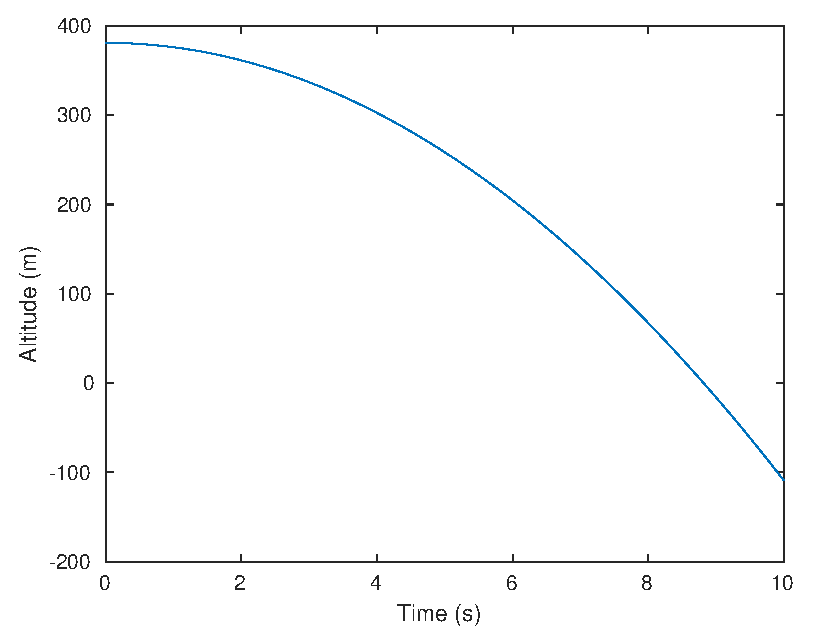
\includegraphics[height=3in]{book/figs/penny.eps}}
\caption{Altitude versus time for an object in free fall.}
\label{fig:penny}
\end{figure}

Figure~\ref{fig:penny} shows the result.  Altitude drops slowly at first and picks up speed.  Between 8 and 9 seconds, the altitude reaches 0, which means the penny hits the sidewalk.  But {\tt ode45} doesn't know where the ground is, so the penny keeps going through zero into negative altitude.  We can solve that problem using events.


\section{ODE events}
\label{events}

\index{ODE events}

Normally when you call {\tt ode45} you specify a start time and
an end time.  But sometimes you don't know ahead of time when the
simulation should end.  MATLAB provides a way to deal with this problem; here's how it works:

\index{event function}
\index{function!event}
\index{ODE event}

\begin{enumerate}

\item Define an {\bf event function} that specifies when the simulation should stop.  For example,  here is an event function for the penny example:

\begin{code}
function [value, isterminal, direction] = event_func(t,X)
    value = X(1);
    isterminal = 1;
    direction = -1;
end
\end{code}

The event function takes the the same input variables as the rate function and returns three output variables: {\tt value} determines whether an {\bf event} can occur, {\tt direction} determines whether it does, and {\tt isterminal} determines what happens.

An event can occur when {\tt value} passes through 0.
If {\tt direction} is positive, the event only occurs if {\tt value} is increasing.
If {\tt direction} is negative, the event only occurs if {\tt value} is decreasing.
If {\tt direction} is 0, the event always occurs.

If {\tt isterminal} is 1, the event causes the simulation to end; otherwise the simulation continues.

This event function uses the altitude of the penny as {\tt value}, so an event occurs when the altitude is decreasing and passes through 0.  When it does, the simulation ends.

\index{odeset@{\tt odeset}}
\index{options@{\tt options}}

\item Use {\tt odeset} to create an object called {\tt options}:

\begin{code}
options = odeset('Events', @event_func);
\end{code}
%
The name of the option is {\tt Events} and the value is the handle of the event function.  

\item Pass {\tt options} as a fourth argument to {\tt ode45}:

\begin{code}
[T, M] = ode45(@rate_func, tspan, X, options);
\end{code}

When {\tt ode45} runs, it invokes \verb"event_func" after each timestep.  If the event function indicates that a terminal event occurred, 
{\tt ode45} stop the simulation.

\end{enumerate}

Let's look at the results from the penny example.  

\begin{code}
>> T(end)
8.8179

>> M(end, :)
0.0000  -86.4153
\end{code}

The last value of {\tt T} is 8.817, which is the number of seconds the penny takes to reach the sidewalk.

The last row of {\tt M} indicates that the final altitude is 0, which is what we wanted, and the final velocity is about \SI{86}{\meter \per \second}.


\section{Air resistance}
\label{air_resistance}

\index{drag}
\index{air resistance}

To make this simulation more realistic, we can add air resistance.
For large objects moving quickly through air, the force due to air resistance, called ``drag'', is proportional to velocity squared.  
For an object falling down, drag is
directed up, so if velocity is negative, drag force is positive.

\begin{equation}
    f_d = -sgn(v) b v^2 
\end{equation}

where $v$ is velocity and
$b$ is a drag constant that depends on the density of
air, the cross-sectional area of the object and the shape
of the object.  

% b is used in the book "Physics for Scientists and Engineers" by Paul A. Tipler.

%TODO: revert this

$sgn$ is the sign or signum function, which is 1 for positive values of 
$v$ and -1 for negative values.  So $f_d$ is always in the opposite direction of $v$.

\index{signum function}
\index{sgn@{\tt sgn}}
\index{mass}
\index{terminal velocity}

To convert from force to acceleration, we have to know mass, but that's easy to find: the mass of a penny is about \SI{2.5}{\gram}.  It's not as easy to find the drag constant, but I have estimated\footnote{Based on reports that the terminal velocity of a penny is about \SI{18}{\meter \per \second}.} that it is about \SI{75e-6}{\kilogram \per \meter}.

Here's a function that takes {\tt t} and {\tt X} as input variables and returns the total acceleration of the penny due to gravity and drag:

\begin{code}
function res = acceleration(t, X)
    b = 75e-6;                % drag constant in kg/m
    v = X(2);                 % velocity in m/s
    f_d = -sgn(v) * b * v^2;  % drag force in N

    m = 2.5e-3;               % mass in kg
    a_d = f_d / m;            % drag acceleration in m/s^2

    a_g = -9.8;               % acceleration of gravity in m/s^2
    res = a_g + a_d;          % total acceleration
end
\end{code}

The first three lines compute force due to drag.
The next two lines compute acceleration due to drag.
The last two lines compute total acceleration due to drag and gravity.

\index{acceleration}
\index{force}

Be careful when you are working with forces and accelerations; make sure
you only add forces to forces or accelerations to accelerations.  In my
code, I use comments to remind myself what units the values are in.
That helps me avoid nonsense like adding forces to accelerations.

To use this function, I made a small change in \verb"rate_func":

\begin{code}
function res = rate_func(t, X)
    y = X(1);      
    v = X(2);      
    
    dydt = v;
    dvdt = acceleration(t, X);   % this line has changed

    res = [dydt; dvdt];
end

\end{code}

\begin{figure}
\centerline{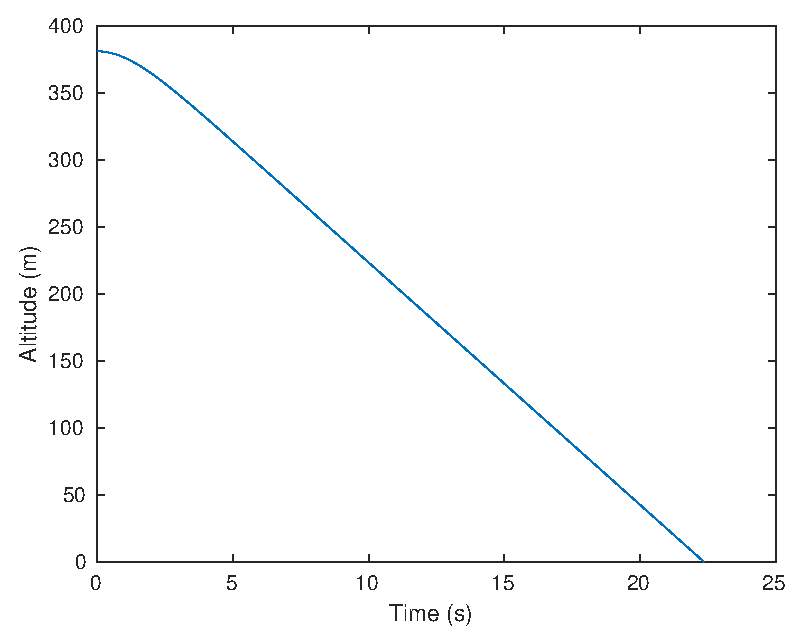
\includegraphics[height=3in]{book/figs/penny2.eps}}
\caption{Altitude versus time for an penny in free fall with air resistance.}
\label{fig:penny2}
\end{figure}

Everything else is the same.  Figure~\ref{fig:penny2} shows the result. 

Air resistance makes a big difference!  Velocity increases until
the drag acceleration equals $g$; after that, velocity is constant and position decreases linearly (and much more slowly than it would in a vacuum).

With air resistance, the time until the penny hits the sidewalk is \SI{22.4}{\second}, substantially longer than before (\SI{8.8}{\second}).

And the final velocity is \SI{18.1}{\meter \per \second}, substantially slower than before (\SI{86}{\meter \per \second}).


%\section{Glossary}
%
%\begin{description}
%
%\item[ODE event:]
%
%\item[event function:]
%
%\end{description}


\section{Exercises}


\begin{ex}

\index{skydiver}
\index{parachute}

The drag constant for a skydiver without a parachute is about \SI{0.2}{\kilogram \meter}.  Modify the penny code from this chapter to simulate the descent of a \SI{75}{\kilogram} skydiver from an initial altitude of \SI{4000}{\meter}.  What is the velocity of the skydiver on impact?

After opening a parachute, the velocity of the skydiver slows to about \SI{5}{\meter\per\second}.  Use your simulation to find the drag constant that yields a terminal velocity of \SI{5}{\meter\per\second}.

Increase the mass of the skydiver, and confirm that terminal velocity increases.  This phenomenon is the source of the intuition that heavy objects fall faster; in air, they do!

Now suppose the skydiver free falls until they get to altitude \SI{1000}{\meter} before opening the parachute.  How long would it take them to reach the ground?

What is the lowest altitude where the skydiver can open the parachute and still land at less than \SI{6}{\meter\per\second} (assuming that the parachute opens and deploys instantly)?

% skydiver.m
\end{ex}



\begin{ex}
\label{earth}

\index{Earth}
\index{Sun}
\index{Law of Universal Gravitation}

Here's a question from the web site {\em Ask an Astronomer}\footnote{\url{https://web.archive.org/web/20180617133223/http://curious.astro.cornell.edu/about-us/39-our-solar-system/the-earth/other-catastrophes/57-how-long-would-it-take-the-earth-to-fall-into-the-sun-intermediate}}:

\begin{quote}
``If the Earth suddenly stopped orbiting the Sun, I know eventually it would be pulled in by the Sun's gravity and hit it. How long would it take the Earth to hit the Sun? I imagine it would go slowly at first and then pick up speed.''
\end{quote}

Use {\tt ode45} to answer this question.  Here are some suggestions about how to proceed:

\begin{enumerate}

\item Look up the Law of Universal Gravitation and any constants you need. I suggest you work entirely in SI units: meters, kilograms, and Newtons.

\item When the distance between the Earth and the Sun gets small, this system behaves badly, so you should use an event function to stop when the surface of Earth reaches the surface of the Sun.

\item Express your answer in days, and plot the results as millions of kilometers versus days.

\end{enumerate}

% earth.m
\end{ex}


% chpt11


\end{document}
